%!TEX ROOT = thesis.tex

\chapter{Semantics Retrieval Engine, Results and Analysis}

\label{section:retrievalengine}
\section{Introduction}

As described in Section \ref{section:introduction}, there's an evident gap between the process of obtaining user described events and the retrieval of the intended video shots. Traditional approach of collecting text-based description of events alone are insufficient for effective retrieval process. With the vehicle-specific features such as the vehicle trajectory, time-stamp information, and color information extracted via the extraction module introduced in Chapter \ref{section:semanticsextraction}, retrieval modules were designed to retrieve video shots that resembles user described queries. This chapter aims to engage the topic of semantic retrieval engines in detail and evaluate their performances along with analysis of the end results.

In this chapter, two retrieval module with relatively different concepts and underlying framework are discussed. The first module was designed with a classic document retrieval system in mind, while the second module was developed in order to address the shortcomings of the first. This is then followed by the methods used to measure the difference between the user-described trajectory, methods used to classify the vehicle color, scoring system used along with the results based on multiple user's review of the proposed method. This chapter also includes the speed measurement of the second retrieval engine.

As a reminder, both the vehicle trajectory and vehicle color evaluation process was separated in order to better gauge the performance of each module (see \ref{sec:expmethodology}).


\cc{please measure the VISER retrieval speed and attach the results.}




\section{\versionOne}
This section uncovers the techniques used behind this retrieval engine's framework along with the results. As previously introduced, as this retrieval engine was inspired by Locality Sensitive Hashing (LSH), documents are hashed into similar locations depending on the similarity. With that in mind, first, the concept of this retrieval engine is discussed. Next, the scoring system is discussed, the evaluation of the system is performed and recorded in the following subsections.




\subsection{Concept}
\label{versionOneConcept}
By taking advantage of the spatio-temporal atom cubes structure introduced in Chapter \ref{section:atoms}, each cataloged event in an atom were treated as an unique document. The underlying atom-based structure allows queries to be formed in a way which emulates the semantics extraction process, hence, eliminating the need for query parsing which in turn reduces the need of both pre- and post-processing of the given queries. 

In this setup, each document that contains similar contents were placed in the same SQL table as a mode of clustering documents. An example is given in Table \ref{table:dbSample} to provide a better visualization of the proposed method. These sequence of events is also visualized in Figure \ref{fig:motionExample} with the trajectory marked with \textcircled{2}. In the example, a red vehicle was detected frame 180 to 184 of a video file on the 19th of March 2016 at 8:51:00am until 8:51:05am, from atom location (3,15) to (5,17) but was detected as a pink vehicle at frame 181. Using Equation \ref{eq:file_timing}, the event's current frame time can be calculated. Given that the current frame is 181, the current frame time would equate to  $(6_{minutes} \times \frac{181}{360}) + 08:48:00am = 8:51:01am$.

As each cataloged event is treated as a unique document (a single record in the database) in this framework, the retrieval process begins by filtering out tables which are irrelevant to the query, $\mathbb{Q}$. Falling back on the example given in Table \ref{table:dbSample}, the system is able to effectively skip through 9 color tables and 5 motion tables, hence speeding up the process to locate documents of interest while reducing the overhead cost involved when going through an entire database. Upon filtering out irrelevant tables, the retrieval engine proceeds to extract and group all the relevant records according to the filenames.

Next, the retrieved results are validated to see if they belong to the same vehicle by cross-checking the obj\_id, along with that, the retrieval engine also performs validation to check if the results belong to a similar time-frame by comparing the t-coordinate. This step is essential to ensure that the results belong to the same vehicle trajectory group as the initial tracker may re-assign a obj\_id to another vehicle during the background subtraction process. While the results returned at this point were accurate, one major problem that occurs using the current process is the low recall rate. The recall rate in a retrieval engine can be thought as the percentage of relevant documents which were retrieved over the total amount of relevant documents; while a low recall rate is preferable in an environment where the accuracy of the retrieved result is regarded with high importance and false negatives are welcomed over false positive such as the medical industry, this was not the case in the proposed method.

In order to overcome the limitation of the low recall rate, a Confidence Value (CV) score parameter was introduced. The CV parameter was used to adjust the sensitivity level of accepting a video shot as part of the final retrieved results. In the proposed method, a lower CV would return a larger set of results at the expense of an increase of retrieved shots which may or may not improve the overall accuracy of the retrieval engine. Each retrieved shot, $\mathbb{S}_i$, will be accepted as the final retrieved results if it fulfills the condition in Equation \ref{eq:CVscore}. The use of the CV score parameter provides a margin of error when performing the query which acts as a trade-off function.

\begin{equation}
\label{eq:CVscore}
CV < \frac{\text{length}(\mathbb{S}_i)}{\text{length}(\mathbb{Q})} \times 100\%
\end{equation}



Upon validating the sanctity of the results, commands were sent to FFmpeg to extract the video shots based on the given filename along with the start and end frame number. Finally, the users are presented with the output from the retrieval engine where the final results can be viewed.


% Please add the following required packages to your document preamble:
% \usepackage[normalem]{ulem}
\begin{table}[hbt]
	\centering 
\caption{Database structure for a vehicle identified as red and pink color with object id "1" of the \versionOne }
\label{table:dbSample}
\begin{tabular}{llllll}
\multicolumn{6}{l}{{ color\_red}} \\ \hline
\multicolumn{1}{|l|}{\textbf{row\_id}} & \multicolumn{1}{l|}{\textbf{filename}}    & \multicolumn{1}{l|}{\textbf{obj\_id}} & \multicolumn{1}{l|}{\textbf{atom\_x}} & \multicolumn{1}{l|}{\textbf{atom\_y}} & \multicolumn{1}{l|}{\textbf{atom\_t}} \\ \hline
\multicolumn{1}{|l|}{n}                & \multicolumn{1}{l|}{20160319\_084800.mp4} & \multicolumn{1}{l|}{1}                & \multicolumn{1}{l|}{3}                & \multicolumn{1}{l|}{15}               & \multicolumn{1}{l|}{180}              \\ \hline
\multicolumn{1}{|l|}{n+1}              & \multicolumn{1}{l|}{20160319\_084800.mp4} & \multicolumn{1}{l|}{1}                & \multicolumn{1}{l|}{3}                & \multicolumn{1}{l|}{16}               & \multicolumn{1}{l|}{182}              \\ \hline
\multicolumn{1}{|l|}{n+2}              & \multicolumn{1}{l|}{20160319\_084800.mp4} & \multicolumn{1}{l|}{1}                & \multicolumn{1}{l|}{4}                & \multicolumn{1}{l|}{16}               & \multicolumn{1}{l|}{183}              \\ \hline
\multicolumn{1}{|l|}{n+3}              & \multicolumn{1}{l|}{20160319\_084800.mp4} & \multicolumn{1}{l|}{1}                & \multicolumn{1}{l|}{5}                & \multicolumn{1}{l|}{17}               & \multicolumn{1}{l|}{184}              \\ \hline
                                       &                                           &                                       &                                       &                                       &                                       \\
\multicolumn{6}{l}{{ color\_pink}}                                                                                                                                                                                                              \\ \hline
\multicolumn{1}{|l|}{\textbf{row\_id}} & \multicolumn{1}{l|}{\textbf{filename}}    & \multicolumn{1}{l|}{\textbf{obj\_id}} & \multicolumn{1}{l|}{\textbf{atom\_x}} & \multicolumn{1}{l|}{\textbf{atom\_y}} & \multicolumn{1}{l|}{\textbf{atom\_t}} \\ \hline
\multicolumn{1}{|l|}{m}                & \multicolumn{1}{l|}{20160319\_084800.mp4} & \multicolumn{1}{l|}{1}                & \multicolumn{1}{l|}{3}                & \multicolumn{1}{l|}{16}               & \multicolumn{1}{l|}{181}              \\ \hline
                                       &                                           &                                       &                                       &                                       &                                       \\
\multicolumn{6}{l}{{ direction\_down}}                                                                                                                                                                                                          \\ \hline
\multicolumn{1}{|l|}{\textbf{row\_id}} & \multicolumn{1}{l|}{\textbf{filename}}    & \multicolumn{1}{l|}{\textbf{obj\_id}} & \multicolumn{1}{l|}{\textbf{atom\_x}} & \multicolumn{1}{l|}{\textbf{atom\_y}} & \multicolumn{1}{l|}{\textbf{atom\_t}} \\ \hline
\multicolumn{1}{|l|}{h}                & \multicolumn{1}{l|}{20160319\_084800.mp4} & \multicolumn{1}{l|}{1}                & \multicolumn{1}{l|}{3}                & \multicolumn{1}{l|}{15}               & \multicolumn{1}{l|}{181}              \\ \hline
                                       &                                           &                                       &                                       &                                       &                                       \\
\multicolumn{6}{l}{{ direction\_motionless}}                                                                                                                                                                                                    \\ \hline
\multicolumn{1}{|l|}{\textbf{row\_id}} & \multicolumn{1}{l|}{\textbf{filename}}    & \multicolumn{1}{l|}{\textbf{obj\_id}} & \multicolumn{1}{l|}{\textbf{atom\_x}} & \multicolumn{1}{l|}{\textbf{atom\_y}} & \multicolumn{1}{l|}{\textbf{atom\_t}} \\ \hline
\multicolumn{1}{|l|}{j}                & \multicolumn{1}{l|}{20160319\_084800.mp4} & \multicolumn{1}{l|}{1}                & \multicolumn{1}{l|}{3}                & \multicolumn{1}{l|}{16}               & \multicolumn{1}{l|}{182}              \\ \hline
                                       &                                           &                                       &                                       &                                       &                                       \\
\multicolumn{6}{l}{{ direction\_right}}                                                                                                                                                                                                         \\ \hline
\multicolumn{1}{|l|}{\textbf{row\_id}} & \multicolumn{1}{l|}{\textbf{filename}}    & \multicolumn{1}{l|}{\textbf{obj\_id}} & \multicolumn{1}{l|}{\textbf{atom\_x}} & \multicolumn{1}{l|}{\textbf{atom\_y}} & \multicolumn{1}{l|}{\textbf{atom\_t}} \\ \hline
\multicolumn{1}{|l|}{k}                & \multicolumn{1}{l|}{20160319\_084800.mp4} & \multicolumn{1}{l|}{1}                & \multicolumn{1}{l|}{3}                & \multicolumn{1}{l|}{16}               & \multicolumn{1}{l|}{183}              \\ \hline
                                       &                                           &                                       &                                       &                                       &                                       \\
\multicolumn{6}{l}{{ direction\_right\_down}}                                                                                                                                                                                                   \\ \hline
\multicolumn{1}{|l|}{\textbf{row\_id}} & \multicolumn{1}{l|}{\textbf{filename}}    & \multicolumn{1}{l|}{\textbf{obj\_id}} & \multicolumn{1}{l|}{\textbf{atom\_x}} & \multicolumn{1}{l|}{\textbf{atom\_y}} & \multicolumn{1}{l|}{\textbf{atom\_t}} \\ \hline
\multicolumn{1}{|l|}{l}                & \multicolumn{1}{l|}{20160319\_084800.mp4} & \multicolumn{1}{l|}{1}                & \multicolumn{1}{l|}{3}                & \multicolumn{1}{l|}{16}               & \multicolumn{1}{l|}{184}              \\ \hline
\end{tabular}
\end{table}

\subsection{Search Interface}

The proposed retrieval engine was realized in a form of a graphical user search interface written in C++, where users are able to construct queries by drawing the trajectory on the interface and providing complementary query information such as the vehicle color. With these user-described query information, the user can then perform queries and obtain the results within seconds. Figure \ref{fig:versionOneInterface} shows the proposed interface with the green lines indicating the user-described trajectory as the query. Upon processing the results, FFmpeg will then extract the video shots and populate the results in a folder.





\begin{figure}[htb!]
	\centering
	\begin{tabular}{c}
		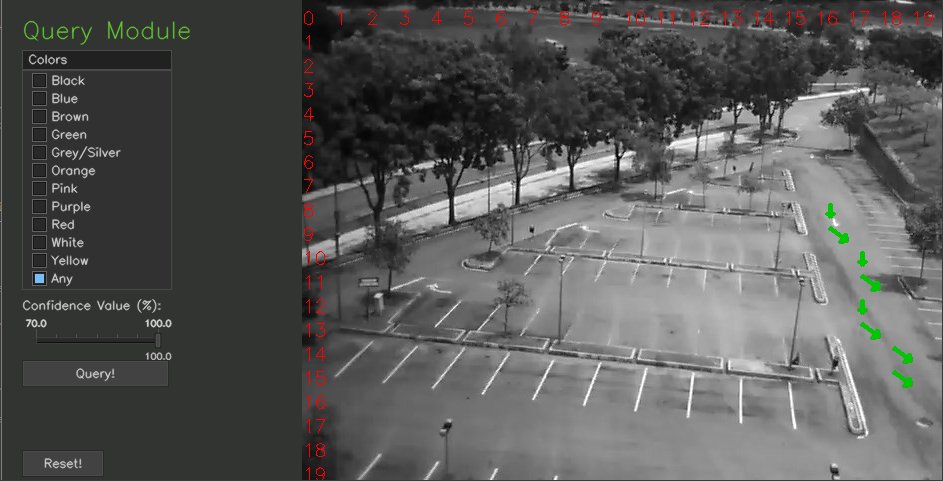
\includegraphics[width=0.7\linewidth]{image/retrievalOne/test1-8inputs.PNG} \\  
		(a) Motion Test Case 1 (TQ1) \\
		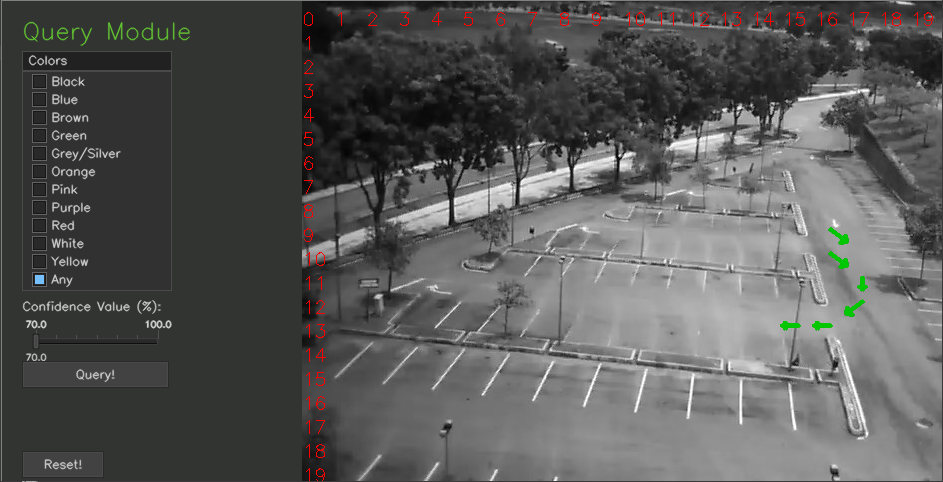
\includegraphics[width=0.7\linewidth]{image/retrievalOne/test2-6input.PNG}\\
		(b) Motion Test Case 2 (TQ2)
	\end{tabular}
	\caption{Search interface for \versionOne} 
	\label{fig:versionOneInterface}
\end{figure}




\subsection{Results and Analysis}
The following subsections describes the evaluation process of the proposed method in Section \ref{section:semantic_lsh} which includes both the vehicle trajectory as well as the vehicle color. As previously mentioned in Section \ref{sec:expmethodology}, only two days of data were fully annotated with the number of vehicles with their corresponding color (see Table \ref{table:colorDist}) as well as the total number of vehicles that performed both $TQ1$ and $TQ2$. 

With the annotated values, the Precision and Recall (Equation \ref{eq:precisionrecall}) metrics were used to measure the performance of the proposed method. These values can be calculated as the total number of event occurrence were recorded; hence, the $F_1$ score can also be computed (Equation \ref{eq:f1score}). The precision of a retrieval engine can be thought as the ratio between number of accurate results over the total number of retrieved results. The recall, on the hand, indicates the ratio of relevant results which were retrieved over the total retrieved results. Finally, the $F_1$ score is used as a harmonic mean between both Precision and Recall values which are both desirable in a retrieval engine.

\begin{align}
\label{eq:precisionrecall}
    \text{Precision} = \frac{tp}{tp + fp}   \hspace{1em} \text{ ; }  \hspace{1em} \text{Recall}  = \frac{tp}{tp + fn}
\end{align}
\begin{align}
\label{eq:f1score}
\text{F1-score}  = 2\cdot\frac{\text{Precision} \cdot \text{Recall}}{\text{Precision} + \text{Recall}}
\end{align}



\subsubsection{Vehicle Trajectory}

In order to evaluate the performance of the retrieval engine in regards to vehicle trajectories, as the manual annotation of these video data is laborous and time consuming, only two specific motion paths were designated as trajectory queries (TQ). The first query, TQ1 refers to vehicles heading southward (see Figure \ref{fig:versionOneInterface} (a)) while TQ2 represents vehicles turning into a junction (see Figure \ref{fig:versionOneInterface} (b)). 

These predefined trajectory queries (TQ) were selected to represent two types of motion which exist in a carpark scene, (i) \textit{simple motion} - motions that are simple in nature, moving straight \& (ii) \textit{complex motion} - motions which contains multiple elements such as turning into a junction. The distribution of these TQ are tabulated in Table \ref{table:motiondist}. In each TQ experiment, the number of atom input query used to represent each TQ were varied to understand the co-relating effects between the number of inputs and the performance of the retrieval engine. In addition to that, the effects of using varying confidence values (CV) in regards to the performance is also evaluated. These experiments were tested on three CV values which were set at 70\%, 80\%, and 90\%.


\begin{table}[bht!]
\centering
\caption{Ground truth distribution of Trajectory Queries}
\label{table:motiondist}
\begin{tabular}{cccc}
\toprule
Trajectory Query &  Trajectory Type & \# of Occurrence & Percentage (\%)   \\
\midrule
TQ1       & Simple Motion       & 252 & 86.3 \%  \\
TQ2      & Complex Motion       & 40 & 13.7\%  \\
\bottomrule
\end{tabular}
\end{table}

Based on the results tabulated in Table \ref{table:motionResults}, the average precision of both TQ1 and TQ2 using CV at 70\% is 67.64\%. The increase of CV to 70\% to 90\% shows an increase in terms of average precision. For TQ1, the average precision increased from 89.50\% to 89.51\% and finally 90.49\% when CV was set at 90\% with a total increase of approximately 1\% for the precision metrics. Likewise, for TQ2, the average precision showed a total increase of 7.44\% when then CV parameter was tweaked. The average precision increased from 45.79\% to 52.61\% and reaching 53.23\% when CV was set to 90\%. 

However, the recall metrics showed a different side of the story when the average recall rate fell from 39.67\% to 18.01\% for TQ1 and 68.15\% to 51.85\% for TQ2. This drastic drop in for recall metrics shows direct co-relation with the requirement of fulfilling Equation \ref{eq:CVscore} for each retrieved shots. The results shows consistency throughout the various experimental settings and true towards the concept which was introduced in \ref{versionOneConcept}.  

As a whole, the $F_1$ score metric was used to evaluate the overall performance of the proposed method as it provides a balance between both of the desirable metrics discussed above. Based on the results, queries with the lowest CV and lower number of inputs tend to perform better than the other parameter settings. The proposed method was able to achieve an $F_1$ score of 74.32\% and 68.08\% for both TQ1 and TQ2. 


\begin{table}[tb!]
\centering
\caption{Results of motion retrieval task with varying CV and number of atom inputs}
\label{table:motionResults}
\vspace{0.5em}
\resizebox{\textwidth}{!}{
\begin{tabular}{ccc|c|c|c|c|c|c|c|c|c|}
\cline{4-12}
\cline{4-12} 
& & & \multicolumn{3}{c|}{CV: 70\%} & \multicolumn{3}{c|}{CV: 80\%} & \multicolumn{3}{c|}{CV: 90\%} \\ \cline{4-12} 
 & & & Precision & Recall & F1 Score & Precision & Recall & F1 Score & Precision & Recall & F1 Score \\ \hline
\multicolumn{1}{|c|}{\multirow{7}{*}{\rotatebox[origin=c]{90}{No. of Input}}} & \multicolumn{1}{c|}{\multirow{4}{*}{\rotatebox[origin=c]{90}{TQ1}}} & 5 & 93.82 & 61.53  & \cellcolor[HTML]{32CB00}\textbf{74.32} & 95.34 & 33.19  & 49.24 & 95.34 & 33.19 & 49.24   \\ \cline{3-12} 
\multicolumn{1}{|c|}{} & \multicolumn{1}{c|}{} & 6 & 90.09 & 36.84 & 52.29 & 90.09 & 36.84  & 52.29 & 89.13 & 16.59 & 27.98    \\ \cline{3-12} 
\multicolumn{1}{|c|}{} & \multicolumn{1}{c|}{} & 7 & 87.27 & 38.86 & 53.78 & 88 & 17.81  & 29.62 & 87.87 & 11.74 & 20.71    \\ \cline{3-12} 
\multicolumn{1}{|c|}{} & \multicolumn{1}{c|}{} & 8 & 86.88 & 21.45 & 34.41 & 84.61 & 13.36  & 23.07 & 89.65 & 10.52 & 18.84    \\ \cline{2-12} 
\multicolumn{1}{|c|}{} & \multicolumn{1}{c|}{\multirow{3}{*}{\rotatebox[origin=c]{90}{TQ2}}} & 4 & 16.28 & 80 & 27.06 & 28.69 & 73.33  & 41.25    & 28.69 & 73.33 & 41.25    \\ \cline{3-12} 
\multicolumn{1}{|c|}{} & \multicolumn{1}{c|}{} & 5 & 65.3 & 71.11  & \cellcolor[HTML]{32CB00}\textbf{68.08} & 73.33 & 48.88  & 58.66 & 73.33 & 48.88  & 58.66    \\ \cline{3-12} 
\multicolumn{1}{|c|}{} & \multicolumn{1}{c|}{} & 6 & 55.81 & 53.33 & 54.54 & 55.81 & 53.33 & 54.54 & 57.69 & 33.33 & 42.25    \\ \hline
\end{tabular}}
\end{table}




\subsubsection{Vehicle Color}

\begin{table}[bht!]
\centering
\caption{Ground truth distribution vehicle colors ordered by occurrence}
\label{table:colorDist}
\begin{tabular}{ccc}
\toprule
Color Term & \# of Occurrence & Percentage (\%)   \\
\midrule
Gray       & 365       & 43.61  \\
Black      & 182       & 21.74  \\
White      & 150       & 17.92  \\
Red        & 60        & 7.17   \\
Blue       & 19        & 2.27   \\
Orange     & 15        & 1.79   \\
Yellow     & 13        & 1.55   \\
Green      & 10        & 1.19   \\
Pink       & 9         & 1.08   \\
Purple     & 7         & 0.84   \\
Brown      & 7         & 0.84   \\
\bottomrule
\end{tabular}
\end{table}




The results of the proposed color term extraction algorithm (\ref{algo:colorExtract}) is tabulated in Table \ref{table:colorMatrix} in a form of a confusion matrix. The cells which are marked in green refers to vehicles which were correctly predicted with the highest count, while cells which are marked in red refers to the highest count of incorrect predictions. The overall performance in terms of precision is around 54\% while the recall is reported at around 36\% with the $F_1$ score of 39\%. The tabulated results also shows that approximately 12\% of vehicles were wrongly classified as achromatic vehicles which were affected by the proposed $T_{pivot}$ value. However, when setting aside the performance of the algorithm to differentiate between chromatic and achromatic vehicles, the proposed method was able to predict the color classes for seven out of eleven color classes. Nevertheless, the results were taken with a grain of salt as the number of test case for each of those color classes were rather low for a decisive verdict. 

Next, the performance of the proposed Algorithm \ref{algo:achromatic} using white and black filters as an approach towards differentiating between all three achromatic colors was analyzed. The proposed algorithm performed relatively well with an average accuracy of 68\%. The results shows that the proposed algorithm did not have much trouble differentiating between black and white vehicles, however, the algorithm tend to have trouble classifying between gray-black and gray-white vehicles as they tend to be ambiguous depending on the lighting condition in the video data. As mentioned above, the $T_{pivot}$'s performance was not up to par. The pivoting process between chromatic and achromatic vehicles proves to be inefficient in harsh lighting condition where shadows and rain would drastically affect the outcome as vehicles may suffer from the lack of chromatic hues which is used to assist in the accurate prediction.

While better results could potentially be obtained by carefully and systematically tweaking the $T_{pivot}$ to perform better at distinguishing between chromatic and achromatic vehicles, the hand crafted parameter may not work well in other scenarios belonging to other dataset, hence, making it undesirable as it is not easily extensible. Another disadvantage of the proposed method used in this framework is that each color had only one final predicted color term. As an example, the predicted results for Red color in Table \ref{table:colorMatrix} illustrates this issue where the color term of three vehicles were assigned Pink instead of Red even though Red and Pink color both belongs to the similar hues. 


\begin{table}[]
\centering
\caption{Confusion matrix for color retrieval task}
\vspace{1.5em}
\label{table:colorMatrix}
\resizebox{\columnwidth}{!}{
\begin{tabular}{ccccccccccccc}
\cline{3-13}
 & \multicolumn{1}{l|}{} & \multicolumn{11}{c|}{Predicted Color} \\ \cline{3-13} 
 & \multicolumn{1}{c|}{} & \multicolumn{1}{c|}{Gray} & \multicolumn{1}{c|}{Black} & \multicolumn{1}{c|}{White} & \multicolumn{1}{c|}{Red} & \multicolumn{1}{c|}{Blue} & \multicolumn{1}{c|}{Orange} & \multicolumn{1}{c|}{Yellow} & \multicolumn{1}{c|}{Green} & \multicolumn{1}{c|}{Pink} & \multicolumn{1}{c|}{Purple} & \multicolumn{1}{c|}{Brown} \\ \hline
\multicolumn{1}{|l|}{} & \multicolumn{1}{c|}{Gray} & \multicolumn{1}{c|}{\cellcolor[HTML]{32CB00}\textbf{236}} & \multicolumn{1}{c|}{61} & \multicolumn{1}{c|}{68} & \multicolumn{1}{c|}{0} & \multicolumn{1}{c|}{0} & \multicolumn{1}{c|}{0} & \multicolumn{1}{c|}{0} & \multicolumn{1}{c|}{0} & \multicolumn{1}{c|}{0} & \multicolumn{1}{c|}{0} & \multicolumn{1}{c|}{0} \\ \cline{2-13} 
\multicolumn{1}{|l|}{} & \multicolumn{1}{c|}{Black} & \multicolumn{1}{c|}{48} & \multicolumn{1}{c|}{\cellcolor[HTML]{32CB00}\textbf{134}} & \multicolumn{1}{c|}{0} & \multicolumn{1}{c|}{0} & \multicolumn{1}{c|}{0} & \multicolumn{1}{c|}{0} & \multicolumn{1}{c|}{0} & \multicolumn{1}{c|}{0} & \multicolumn{1}{c|}{0} & \multicolumn{1}{c|}{0} & \multicolumn{1}{c|}{0} \\ \cline{2-13} 
\multicolumn{1}{|l|}{} & \multicolumn{1}{c|}{White} & \multicolumn{1}{c|}{26} & \multicolumn{1}{c|}{4} & \multicolumn{1}{c|}{\cellcolor[HTML]{32CB00}\textbf{120}} & \multicolumn{1}{c|}{0} & \multicolumn{1}{c|}{0} & \multicolumn{1}{c|}{0} & \multicolumn{1}{c|}{0} & \multicolumn{1}{c|}{0} & \multicolumn{1}{c|}{0} & \multicolumn{1}{c|}{0} & \multicolumn{1}{c|}{0} \\ \cline{2-13} 
\multicolumn{1}{|l|}{} & \multicolumn{1}{c|}{Red} & \multicolumn{1}{c|}{27} & \multicolumn{1}{c|}{25} & \multicolumn{1}{c|}{0} & \multicolumn{1}{c|}{2} & \multicolumn{1}{c|}{0} & \multicolumn{1}{c|}{0} & \multicolumn{1}{c|}{0} & \multicolumn{1}{c|}{0} & \multicolumn{1}{c|}{4} & \multicolumn{1}{c|}{\cellcolor[HTML]{FE0000}\textbf{2}} & \multicolumn{1}{c|}{0} \\ \cline{2-13} 
\multicolumn{1}{|l|}{} & \multicolumn{1}{c|}{Blue} & \multicolumn{1}{c|}{3} & \multicolumn{1}{c|}{10} & \multicolumn{1}{c|}{0} & \multicolumn{1}{c|}{0} & \multicolumn{1}{c|}{\cellcolor[HTML]{32CB00}\textbf{6}} & \multicolumn{1}{c|}{0} & \multicolumn{1}{c|}{0} & \multicolumn{1}{c|}{0} & \multicolumn{1}{c|}{0} & \multicolumn{1}{c|}{0} & \multicolumn{1}{c|}{0} \\ \cline{2-13} 
\multicolumn{1}{|l|}{} & \multicolumn{1}{c|}{Orange} & \multicolumn{1}{c|}{8} & \multicolumn{1}{c|}{3} & \multicolumn{1}{c|}{0} & \multicolumn{1}{c|}{0} & \multicolumn{1}{c|}{0} & \multicolumn{1}{c|}{\cellcolor[HTML]{32CB00}\textbf{3}} & \multicolumn{1}{c|}{0} & \multicolumn{1}{c|}{0} & \multicolumn{1}{c|}{0} & \multicolumn{1}{c|}{1} & \multicolumn{1}{c|}{0} \\ \cline{2-13} 
\multicolumn{1}{|l|}{} & \multicolumn{1}{c|}{Yellow}    & \multicolumn{1}{c|}{3} & \multicolumn{1}{c|}{1} & \multicolumn{1}{c|}{2} & \multicolumn{1}{c|}{0} & \multicolumn{1}{c|}{0} & \multicolumn{1}{c|}{0} & \multicolumn{1}{c|}{\cellcolor[HTML]{32CB00}\textbf{7}} & \multicolumn{1}{c|}{0} & \multicolumn{1}{c|}{0} & \multicolumn{1}{c|}{0} & \multicolumn{1}{c|}{0} \\ \cline{2-13} 
\multicolumn{1}{|l|}{} & \multicolumn{1}{c|}{Green} & \multicolumn{1}{c|}{5} & \multicolumn{1}{c|}{1} & \multicolumn{1}{c|}{4} & \multicolumn{1}{c|}{0} & \multicolumn{1}{c|}{0} & \multicolumn{1}{c|}{0} & \multicolumn{1}{c|}{0} & \multicolumn{1}{c|}{\cellcolor[HTML]{C0C0C0}\textbf{0}} & \multicolumn{1}{c|}{0} & \multicolumn{1}{c|}{0} & \multicolumn{1}{c|}{0} \\ \cline{2-13} 
\multicolumn{1}{|l|}{} & \multicolumn{1}{c|}{Pink} & \multicolumn{1}{c|}{1} & \multicolumn{1}{c|}{0} & \multicolumn{1}{c|}{0} & \multicolumn{1}{c|}{\cellcolor[HTML]{FE0000}\textbf{3}} & \multicolumn{1}{c|}{0} & \multicolumn{1}{c|}{0} & \multicolumn{1}{c|}{0} & \multicolumn{1}{c|}{0} & \multicolumn{1}{c|}{\cellcolor[HTML]{32CB00}\textbf{5}} & \multicolumn{1}{c|}{0} & \multicolumn{1}{c|}{0} \\ \cline{2-13} 
\multicolumn{1}{|l|}{} & \multicolumn{1}{c|}{Purple} & \multicolumn{1}{c|}{3} & \multicolumn{1}{c|}{3} & \multicolumn{1}{c|}{0} & \multicolumn{1}{c|}{0} & \multicolumn{1}{c|}{0} & \multicolumn{1}{c|}{0} & \multicolumn{1}{c|}{0} & \multicolumn{1}{c|}{0} & \multicolumn{1}{c|}{0} & \multicolumn{1}{c|}{1} & \multicolumn{1}{c|}{0} \\ \cline{2-13} 
\multicolumn{1}{|l|}{\multirow{-11}{*}{\rotatebox[origin=c]{90}{Actual Color}}} & \multicolumn{1}{c|}{Brown} & \multicolumn{1}{c|}{3} & \multicolumn{1}{c|}{4} & \multicolumn{1}{c|}{0} & \multicolumn{1}{c|}{0} & \multicolumn{1}{c|}{0} & \multicolumn{1}{c|}{0} & \multicolumn{1}{c|}{0} & \multicolumn{1}{c|}{0} & \multicolumn{1}{c|}{0} & \multicolumn{1}{c|}{0} & \multicolumn{1}{c|}{\cellcolor[HTML]{C0C0C0}\textbf{0}} \\ \hline
 & \multicolumn{1}{l}{} & \multicolumn{1}{l}{} & \multicolumn{1}{l}{} & \multicolumn{1}{l}{} & \multicolumn{1}{l}{} & \multicolumn{1}{l}{} & \multicolumn{1}{l}{} & \multicolumn{1}{l}{} & \multicolumn{1}{l}{} & \multicolumn{1}{l}{} & \multicolumn{1}{l}{} & \multicolumn{1}{l}{} \\ \hline
\multicolumn{1}{|l|}{} & \multicolumn{1}{c|}{Precision} & \multicolumn{1}{c|}{65.01} & \multicolumn{1}{c|}{54.47}                                & \multicolumn{1}{c|}{61.86} & \multicolumn{1}{c|}{40.00} & \multicolumn{1}{c|}{100.00} & \multicolumn{1}{c|}{100.00}                             & \multicolumn{1}{c|}{100.00} & \multicolumn{1}{c|}{N/A} & \multicolumn{1}{c|}{55.56} & \multicolumn{1}{c|}{25.00}                              & \multicolumn{1}{c|}{N/A} \\ \cline{2-13} 
\multicolumn{1}{|l|}{} & \multicolumn{1}{c|}{Recall} & \multicolumn{1}{c|}{64.66} & \multicolumn{1}{c|}{73.63} & \multicolumn{1}{c|}{80.00} & \multicolumn{1}{c|}{3.33} & \multicolumn{1}{c|}{31.58} & \multicolumn{1}{c|}{20.00} & \multicolumn{1}{c|}{53.85} & \multicolumn{1}{c|}{0.00} & \multicolumn{1}{c|}{55.56} & \multicolumn{1}{c|}{14.29} & \multicolumn{1}{c|}{0.00} \\ \cline{2-13} 
\multicolumn{1}{|l|}{\multirow{-3}{*}{\rotatebox[origin=c]{90}{Result}}} & \multicolumn{1}{c|}{F1 Score}  & \multicolumn{1}{c|}{64.84} & \multicolumn{1}{c|}{62.62} & \multicolumn{1}{c|}{69.77} & \multicolumn{1}{c|}{6.15} & \multicolumn{1}{c|}{48.00} & \multicolumn{1}{c|}{33.33} & \multicolumn{1}{c|}{70.00} & \multicolumn{1}{c|}{N/A} & \multicolumn{1}{c|}{55.56} & \multicolumn{1}{c|}{18.18} & \multicolumn{1}{c|}{N/A} \\ \hline
\end{tabular}%
}
\end{table}


% However, the current implementation of the proposed method search interface has yet to include time slicing query options. 

%However, should the initial test against the $T_{pivot}$ fails, the proposed method is able to fall back on the HSV histogram results.


\section{\versionTwo}

This section expounds on the techniques used behind this retrieval engine's framework along with the results. The proposed interface in \versionTwo also focuses on extensibility as well as ease of access of the retrieval engine while improving on the overall results. The JavaScript (JS) language was selected as a means to this end as it is commonly used in web browsers. The focus of this work sees a shift from indexing methods to results-sorting optimization by measuring the difference between the query and the retrieved results. The concept and scoring systems used in this retrieval engine will be discussed further in the following subsections along with the evaluation. 

\subsection{Concept}

Instead of treating each spatio-temporal atom cubes as an unique document, in this framework, the unique identifiers ($atom_x$, $atom_y$, $atom_t$) of each atom was used for the retrieval process. As mentioned above, the focus of this framework veered towards the use of distance measures (see Section \ref{section:distancemeasures}) and its applications in order to retrieve results that are relevant.

In the same manner, the graphical input query was designed in such a way that it takes on the properties of the atom cubes' unique identifiers with the exception of the $atom_t$. As a substitute of the identifier, the order of the input, $o_{i}$, was used as a replacement. This was possible as the order was used to mimic the motion of the target vehicle shot. However, to do so, first, the graphical query input needs to be converted into a set, $\mathbb{Q}$, by removing duplicate identifiers which was introduced by the mouse stroke. This will thus result with unique identifiers remaining in the set. 

As the retrieval engine deals with a huge set of data, the next logical step was to find ways to optimize and minimize the search scope. In this framework, a simplistic approach was taken to further narrow down the search scope. 
The time and date semantics were utilized as these useful metadata which were extracted during the semantic extraction phase were suitable candidates in assisting the filtering process. 
Equation \ref{eq:timedatefilter} was used to filter out records from the database which does not fulfill the input query's requirements and include records $\mathbb{R}$ which made it into set $\mathbb{P}$. 



\begin{gather} 
\label{eq:timedatefilter}
     \text{Start Timestamp} \hspace{.5em} \leq \hspace{.5em} \mathbb{R}[i] \hspace{.5em} \leq \hspace{.5em} \text{End Timestamp} \hspace{.5em} \Rightarrow \hspace{.5em} \mathbb{R}[i] \in \mathbb{P} 
\end{gather}   


\cc{rewrite the following part... so messy!}



\begin{equation}
    \mathbb{Q} = \{ (x_i, y_i, o_i), (x_{i+1}, y_{i+1}, o_{i+1}), (x_{i+2}, y_{i+2}, o_{i+2}), \dotsb,(x_{i+n}, y_{i+n}, o_{i+n})\}
\end{equation}



Now, with the output from the filtering process, these records can be compared against the input query $\mathbb{Q}$. This step begins by comparing the length of the query ($\mathbb{Q}_{length}$) against the length of the individual records ($\mathbb{R}[i]_{length}$) in the database. This step is an essential ingredient for the next phase of measuring the dissimilarity using Chamfer Distance.


Chamfer Distance, $D_{chamfer}$, is one of the many distance measure metrics available. $D_{chamfer}$ can be formalized using Equation \ref{eq:chamferDistance}. In this framework, this distance metrics is use to measure the dissimilarity between the input query $\mathbb{Q}$ and each record $\mathbb{R}[i]$ that fulfills the Equation \ref{eq:timedatefilter}, these records will then be included in the $\mathbb{P}$ set. In order to maximize the dissimilarity in Equation \ref{eq:chamferDistance}, the lengths ($\mathbb{Q}_{length}$, $\mathbb{R}[i]_{length}$) are taken into consideration. Based on Equation \ref{eq:chamferDistance}, while all the elements within both the sets will be compared against each other, the final value will be normalized by the length of $P$. 



\begin{equation}
\label{eq:chamferDistance}
D_{Chamfer} (\mathbb{P},\mathbb{Q}) = \frac{1}{\mid P \mid} \sum_{t_p \in \mathbb{P}} \min_{t_q \in \mathbb{Q}}  \mid t_p - t_q \mid^{2}
\end{equation}



\subsection{Scoring System}
\subsection{Vehicle Trajectory}
\subsection{Vehicle Color \& Color Mode}
\subsection{Results}

\section{Result Analysis}
We also note that the achromatic algorithm is an essential step because the 8 Values bins are insufficient to accurately represent vehicles with borderline dominant color as the brightness values may be widely distributed.



\cc{for the analysis, include a "heatmap" of the versionone vs versiontwo for the evaluation of results}


